\documentclass[12pt, oneside]{report}

\usepackage[left=2.5cm, top=2.5cm, bottom=2.5cm, right=2.5cm]{geometry}

\usepackage[utf8]{inputenc}
\usepackage[T1]{polski}
\usepackage[polish]{babel}
\usepackage{hyperref}
\usepackage{physics}
\usepackage{graphicx}
\usepackage{amsthm}
\usepackage{enumitem}
\usepackage{mathtools}
\usepackage{amsfonts}

\newtheorem{theorem}{Twierdzenie}
\newtheorem{lemma}{Lemat}
\newtheorem{definition}{Definicja}
\newcommand\Omicron{O}
\DeclarePairedDelimiter\floor{\lfloor}{\rfloor}

\begin{document}  
\thispagestyle{empty}
\begin{titlepage}
    \begin{center}

           \Large
    \textbf{Uniwersytet Jagielloński w Krakowie}\vspace{0.2cm}\\ Wydział Matematyki i Informatyki
               \vspace*{1cm}
               
         \vspace{3cm}
         \Large
          \textbf{Pola Kyzioł}\\\vspace{0.5cm}
         \normalsize Nr albumu: 1092406\\
             \vspace{2cm}
        \Huge
        \textbf{Algorytmy dynamiczne po dekompozycji drzewowej dla problemów grafowych o spójnych rozwiązaniach.}
      
        \vspace{1.5cm}
        \normalsize
        Praca magisterska\\
        na kierunku Informatyka Analityczna\\ \vspace{0.15cm}
        
        \vfill
        \vspace{2cm}
       \begin{minipage}{1\textwidth}
\begin{flushright}
Praca wykonana pod kierunkiem\\
dr hab. Tomasz Krawczyk\\
Instytut Informatyki Analitycznej 
\end{flushright}
\end{minipage}
        
        \vspace{2cm}
        \begin{center}
      Kraków 2019
        \end{center}
    \end{center}
\end{titlepage}

\newpage 
 \thispagestyle{empty}
\vspace{2.5cm}
\begin{flushleft}
\large \textbf{Oświadczenie autora pracy}\vspace{0.6cm}\\
\end{flushleft}

\noindent Świadom odpowiedzialności prawnej oświadczam, że niniejsza praca dyplomowa została napisana przeze mnie samodzielnie i nie zawiera treści uzyskanych w sposób niezgodny z obowiązującymi przepisami.\\

\noindent Oświadczam również, że przedstawiona praca nie była wcześniej przedmiotem procedur związanych z uzyskaniem tytułu zawodowego w wyższej uczelni.
\vspace{2cm}
\begin{center}
\begin{tabular}{lr}
................................~~~~~~~~~~~~~~~~~~~~~~~~~~~~~~~~~~~~~~&
.......................................... \\
{~~~~Kraków, dnia} & {Podpis autora pracy~~~~}
\end{tabular}
\end{center}
\vspace{5cm}
\begin{flushleft}
\large \textbf{Oświadczenie kierującego pracą}
\end{flushleft}

\noindent Potwierdzam, że niniejsza praca została przygotowana pod moim kierunkiem i~kwalifikuje się do przedstawienia jej w postępowaniu o nadanie tytułu zawodowego.
\vspace{2cm}
\begin{center}
\begin{tabular}{lr}
................................~~~~~~~~~~~~~~~~~~~~~~~~~~~~~~~~~~~~~~&
............................................ \\
{~~~~Kraków, dnia} & {Podpis kierującego pracą~~}
\end{tabular}
\end{center}
\vfill

\newpage
\tableofcontents

\newpage
  	\chapter{Wprowadzenie}
  		
\newpage
  	\chapter{Podstawowe definicje}
	
\begin{definition}
\em \emph{Dekompozycją drzewową grafu} $G$ nazywamy parę $\mathcal{T} = (T, \{X_t : t \in V(T)\})$, gdzie $T$ jest drzewem, a $\{X_t : t \in V(T)\}$ rodziną zbiorów wierzchołków grafu $G$ spełniającą następujące warunki:
\begin{enumerate}[label=(\roman*)]
	\item{Dla każdej krawędzi $\{u, v\} \in E(G)$ istnieje węzeł $t \in V(T)$, taki że $u \in X_t$ i $v \in X_t$.}
	\item{Dla każdego wierzchołka $v \in V(G)$ zbiór $\{t \in V(T): v \in X_t \}$ jest poddrzewem drzewa $T$.}
\end{enumerate}
\end{definition}

Od tej pory wierzchołki grafu $G$ będą nazywane po prostu \emph{wierzchołkami}, natomiast wierzchołki drzewa $T$ będą nazywane \emph{węzłami}.

\begin{definition}
\em \emph{Szerokość drzewowa dekompozycji drzewowej $\mathcal{T}$}, $sd_\mathcal{T}$, opisuje rozmiar najliczniejszego węzła pomniejszony o $1$: $$sd_\mathcal{T} = max_{t \in V(T)} \abs{X_t - 1}$$ 
\end{definition}

\begin{definition}
\em \emph{Szerokość drzewowa grafu $G$}, standardowo oznaczana przez $sd_G$ lub $k$, jest minimalną szerokością drzewową wziętą po wszystkich możliwych dekompozycjach drzewowych $G$: $$sd_G = min \{sd_\mathcal{T}: \mathcal{T} \text{ jest dekompozycją drzewową }G\}$$
\end{definition}

Przy konstruowaniu algorytmów dynamicznych działających po dekompozycji drzewowej grafu, łatwiej jest posługiwać się tzw. \emph{ładną dekompozycją drzewową}.

\begin{definition}
\em \emph{Ładna dekompozycja drzewowa} $\mathcal{T} = (T, \{X_t\}_{t \in V(T)})$ to dekompozycja drzewowa o następujących własnościach:
\begin{enumerate}[label=(\roman*)]
	\item{$T$ jest drzewem ukorzenionym.}
	\item{Każdy węzeł $t \in T$ ma jeden z następujących pięciu typów:}
	\begin{enumerate}[label=\arabic*)]
		\item{$t$ jest \texttt{LIŚCIEM:} $X_t = \emptyset$.}
		\item{$t$ jest węzłem \texttt{WPROWADZAJĄCYM} $v$: $t$ ma o jeden wierzchołek więcej niż jego jedyne dziecko: $X_t = X_{t'} \cup \{v\}$. Każdy wierzchołek $v \in V(G)$, ma co najmniej jeden węzeł wprowadzający.}
		\item{$t$ jest węzłem \texttt{ZAPOMINAJĄCYM} $v$: $t$ ma o jeden wierzchołek mniej niż jego jedyne dziecko: $X_t = X_{t'} \setminus \{v\}$. Jego specjalnym reprezentantem jest korzeń. Dla każdego wierzchołka $v \in V(G)$, istnieje dokładnie jeden węzeł zapominający.}
		\item{$t$ jest węzłem \texttt{SCALAJĄCYM}: $t$ posiada dwoje dzieci: $X_t = X_{t'} = X_{t''}$, scala dwa podgrafy o przecięciu $X_t$.}
		\item{$t$ jest węzłem \texttt{WPROWADZAJĄCYM KRAWĘDŹ} $uv$: $X_t = X_{t'}$, ten typ węzła nie pojawił się w pierwotnej definicji ładnej dekompozycji drzewowej, ale znacząco ułatwia definiowanie algorytmów, które na nich operują. Węzeł wprowadzający uzupełnia reprezentację grafu $G$ w drzewie $T$ o krawędź $uv \in E(G)$, $u \in X_t$ i $v \in X_t$. Dla każdego $uv$ istnieje dokładnie jeden węzeł wprowadzający i - przyjmując bez straty ogólności, $t(u)$ jest przodkiem $t(v)$ (gdzie $t(v)$ to najwyższy węzeł, taki że $v \in X_{t(v)}$) - znajduje się on pomiędzy $t(v)$ a węzłem zapominającym $v$.}
\end{enumerate}
\end{enumerate}
\end{definition}

\begin{definition}
\em Dla węzła $t$, definiujemy $G_t = (V_t, E_t)$, gdzie: 
\begin{itemize}[noitemsep,topsep=5pt,parsep=0pt,partopsep=0pt]
\item[$V_t$]{jest zbiorem wierzchołków wprowadzonych w poddrzewie ukorzenionym w $t$.}
\item[$E_t$]{jest zbiorem krawędzi wprowadzonych w poddrzewie ukorzenionym w $t$.} 
\end{itemize}
\end{definition}

\begin{figure}
\centering
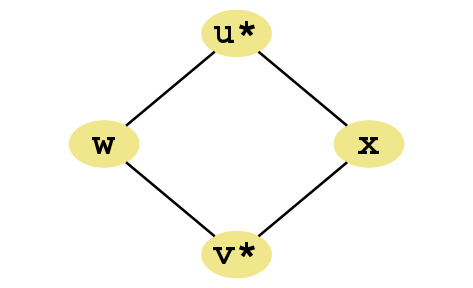
\includegraphics[width=5cm]{square_steiner_tree_standard_graph.png}
\caption{Przykładowy graf $G$.}
\label{kwadrat}
\end{figure}

\begin{figure}
\centering
\makebox[\textwidth]{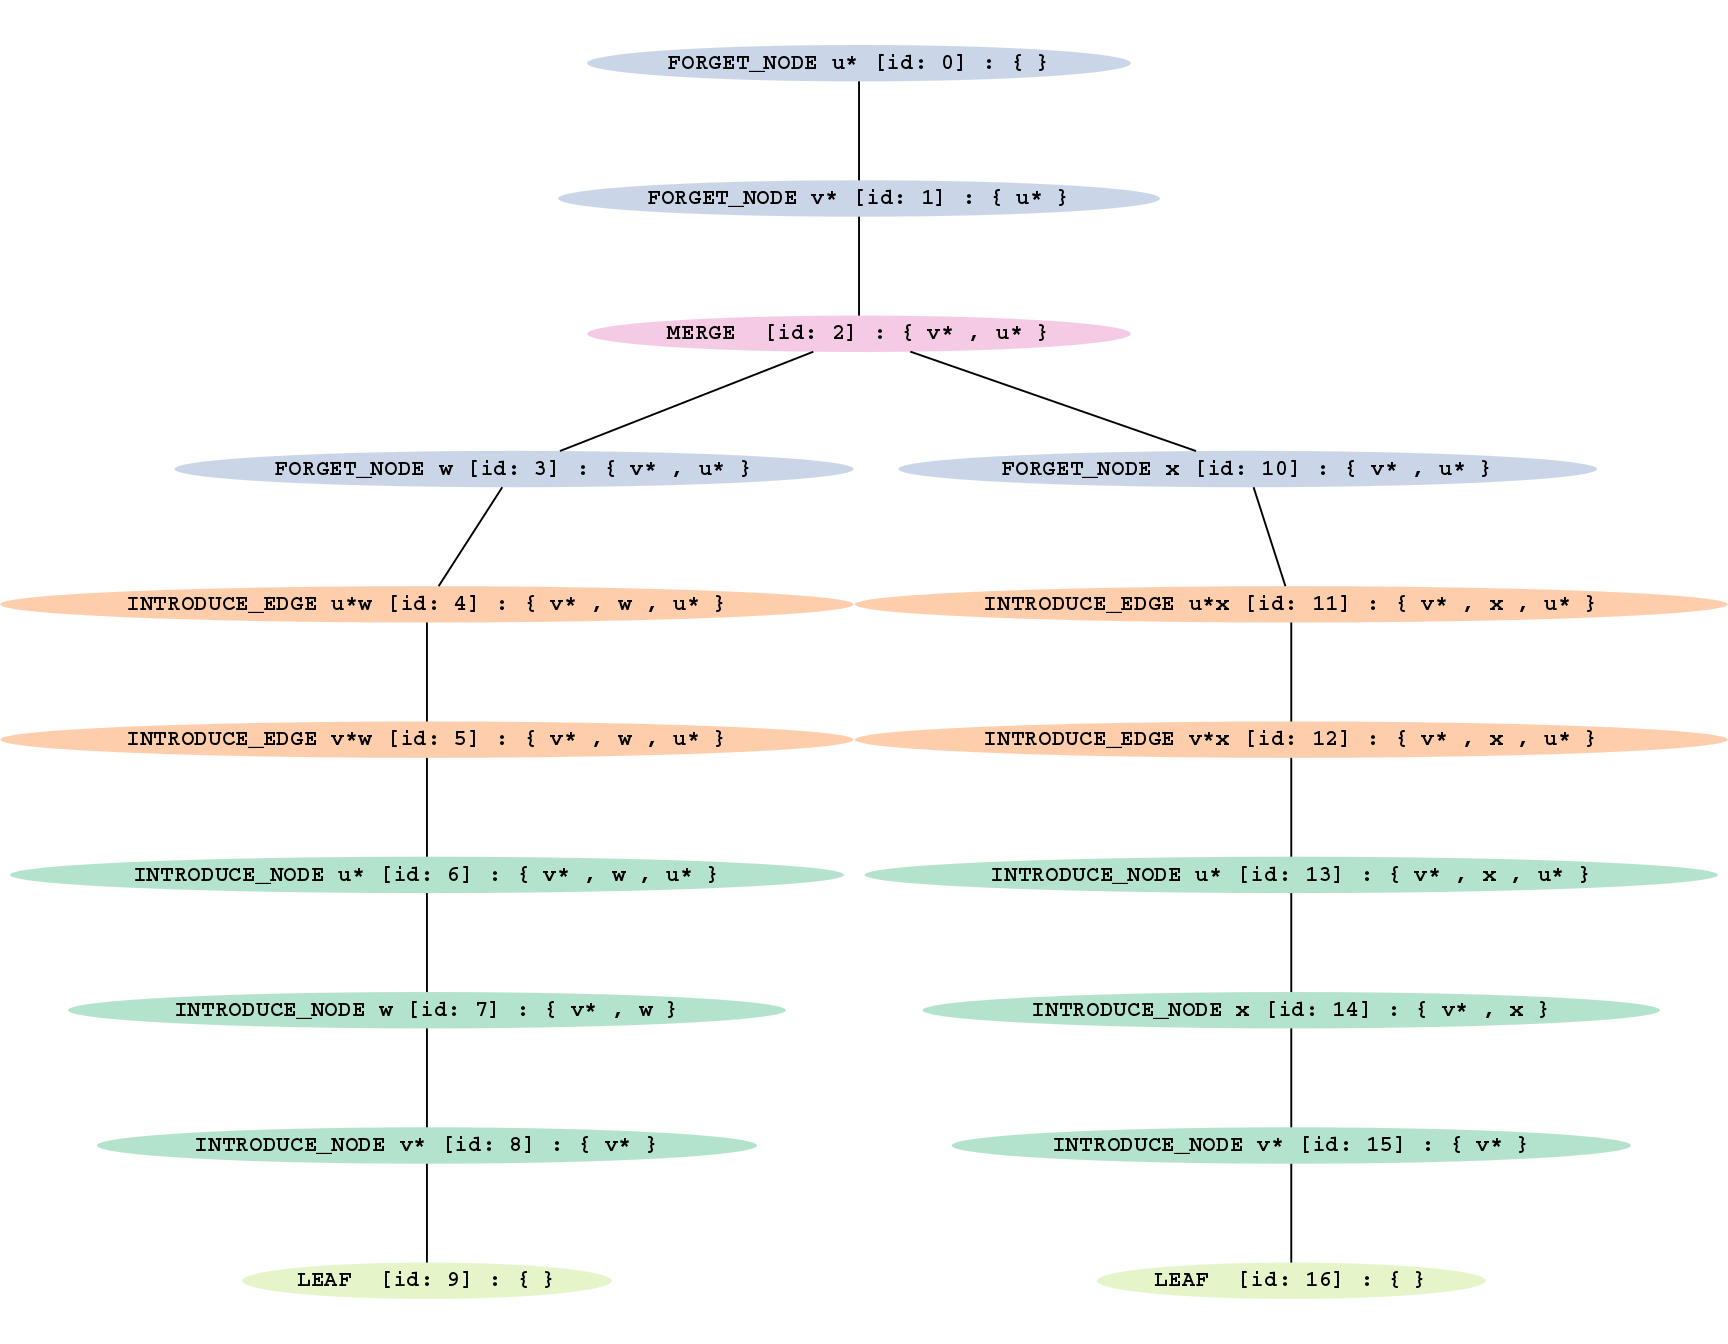
\includegraphics[width=18cm, height=14cm]{square_steiner_tree_standard.png}}
\caption{Ładna dekompozycja drzewowa grafu $G$ z rys. \ref{kwadrat}. Wierzchołki terminalne są oznakowane *.}
\label{dekompozycja_kwadratu}
\end{figure}

Problem obliczania dekompozycji drzewowej należy do klasy problemów FPT. Bodlaender \cite{bodlaender} jako pierwszy podał liniowy algorytm znajdowania dekompozycji drzewowej o szerokości $k$ (o ile taka dekompozycja istnieje). Natomiast Kloks \cite{kloks} pokazał, że dla każdego grafu o szerokości drzewowej $k$ istnieje ładna dekompozycja drzewowa o szerokości drzewowej $k$, którą można skonstruować w czasie liniowym od ilości wierzchołków grafu $G$.

\begin{definition}
\em \emph{Problem Drzewa Steinera.} Na wejściu mamy dany graf $G$ wraz z jego ładną dekompozycją drzewową $\mathcal{T} = (T, \{X_t\}_{t \in V(T)})$, zbiór tzw. terminali $K \subseteq V(G)$ oraz liczbę naturalną $\ell$. Pytamy, czy istnieje spójny graf acykliczny łączący wszystkie terminale o co najwyżej $\ell$ krawędziach potocznie zwany drzewem Steinera.
\end{definition}

\begin{definition}
\em \emph{Problem Cyklu Hamiltona.} Na wejściu mamy dany graf $G$ wraz z jego ładną dekompozycją drzewową $\mathcal{T} = (T, \{X_t\}_{t \in V(T)})$. Pytamy, czy istnieje cykl prosty, który zawiera wszystkie wierzchołki $V(G)$.
\end{definition}

\newpage
  	\chapter{Klasyczne algorytmy dynamiczne}
    	\section{Drzewo Steinera}
    	
W tym rozdziale zostanie przedstawiony klasyczny algorytm dynamiczny po dekompozycji drzewowej dla problemu Drzewa Steinera.

W celu uproszczenia algorytmu, przyjmujemy, że każdy węzeł drzewa $T$ zawiera przynajmniej jeden terminal. Uzyskujemy to, wybierając dowolny wierzchołek $v_0 \in K$ i dodając go do każdego węzła oraz usuwając \texttt{WPROWADZAJĄCY} $v_0$ i \texttt{ZAPOMINAJĄCY} $v_0$. Własności ładnej dekompozycji drzewowej są zachowane z modyfikacją, że liście i korzeń nie są puste.

\begin{figure}
\centering
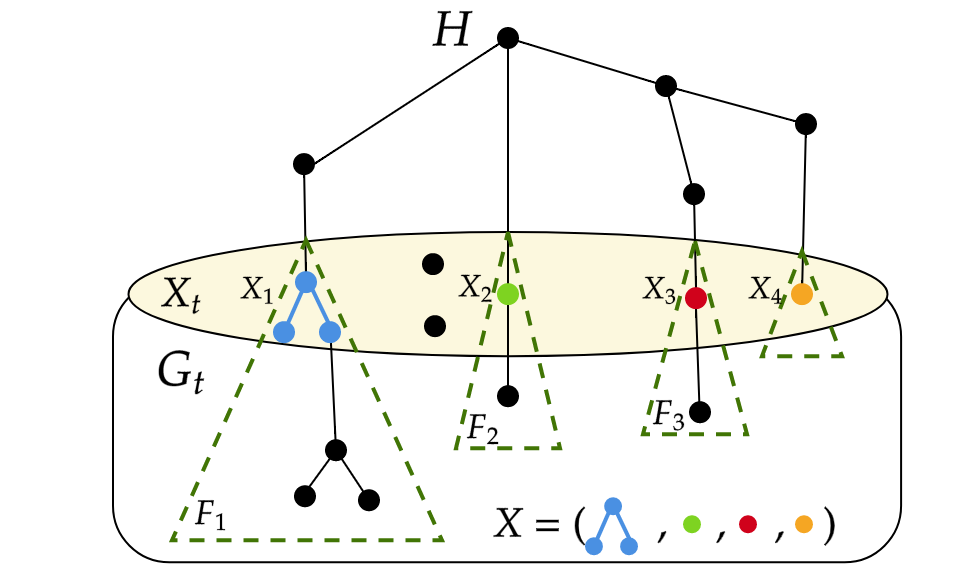
\includegraphics[width=16cm]{steiner_tree.png}
\caption{Opis}
\label{steiner_tree}
\end{figure}

Zastanówmy się, jak wygląda ślad drzewa Steinera w węźle $t$, przykładowy został zobrazowany na rys. Dla $H$ będącego dowolnym drzewem Steinera łączącym wszystkie terminale $K$, przecięcie $H$ i $G_t$ tworzy las $F$, który zawiera przynajmniej jeden wierzchołek terminalny $v_0$. Szukane $H$ jest spójne oraz $X_t$ zawiera terminal, co implikuje, że każde drzewo należące do $F$ przecina $X_t$. Ponadto każdy terminal $v_t \in K \cap V_t$ należy do $F$. Zauważmy, że ślad drzewa Steinera $(X, \mathcal{P})$ w węźle $t$ jest jednoznacznie zdefiniowany przez zbiór wierzchołków $X = V(F) \cap X_t$ oraz jego podział $\mathcal{P} = \{X_1, X_2, \dots, X_z\}$ na zbiory wierzchołków przynależnych do poszczególnych drzew $F$.

Dla każdej trójki $(t, X, \mathcal{P})$ trzymamy w $c(t, X, \mathcal{P})$ rozmiar (liczbę krawędzi) najmniejszego $F$ w $G_t$. Jeśli dana trójka nie spełnia wszystkich warunków $c(t, X, \mathcal{P}) = \infty$. Musimy na bieżąco śledzić partycję $\mathcal{P}$, ponieważ może się ona zmieniać wraz z każdym nowo przetwarzanym węzłem. Węzły \texttt{SCALAJĄCY} lub \texttt{UZUPEŁNIAJĄCY} $uv$ mogą zepsuć wcześniej poprawną partycję, tworząc cykl. Wynik końcowy odpowiada wartości $c(r, \{v_0*\}, \{\{v_0*\}\})$, gdzie $r$ jest korzeniem. Poniżej prezentuję formuły rekurencyjne obliczania wartości $c$ ze względu na typ węzła $t$. Dla wszystkich niewymienionych przypadków, $c$ przyjmuje wartość $\infty$.
\newline\newline
$t$ jest \texttt{LIŚCIEM}
$$c(t, \{v_0*\}, \{\{v_0*\}\}) = 0$$
\newline
$t$ jest węzłem \texttt{WPROWADZAJĄCYM} $v$ - zauważmy, że $v$ nie należał do żadnego z dzieci, wobec czego krawędzie incydentne z $v$ nie zostały jeszcze wprowadzone poprzez węzły wprowadzające i $v$ jest wierzchołkiem izolowanym. Wierzchołek izolowany ma swój własny, jednoelementowy komponent w $\mathcal{P}$. Jeśli $v$ jest terminalem, musi należeć do $X$. Jeśli powyższy warunek jest spełniony: 
\[
c(t, X, \mathcal{P}) =  
\left \{
  \begin{tabular}{ccc}
  $c(t', X \setminus \{v\}, \mathcal{P} \setminus \{\{v\}\})$ & jeśli $v \in X$,\\
  $c(t', X, \mathcal{P})$ & wpp.
  \end{tabular}
\right. 
\]
\newline
t jest węzłem \texttt{WPROWADZAJĄCYM KRAWĘDŹ} $uv$ - mamy 3 przypadki, które rozpatrujemy osobno:

\begin{enumerate}
\item \label{notinx} $u \notin X \lor v \notin X$
\item \label{notinthesamecomponent} $u \in X \land v \in X$ oraz $u$ i $v$ są w różnych komponentach $\mathcal{P}$ ($u \in X_i$, $v \in X_j$, $i \neq j$)
\item \label{edgepossible} $u \in X \land v \in X$ oraz $u$ i $v$ są w tych samych komponentach $\mathcal{P}$ ($u,v \in X_i$)
\end{enumerate} 

W przypadkach \ref{notinx} oraz \ref{notinthesamecomponent} krawędź $uv$ nie może należeć do rozwiązania. Natomiast w przypadku \ref{edgepossible} mamy dwie możliwości - albo włączamy krawędź do rozwiązania, albo nie. Jeśli nie dorzucamy krawędzi do śladu, przepisujemy częściowy wynik z $t'$ dla tej samej partycji. W przeciwnym przypadku, nowo dodawana krawędź musiała połączyć dwa rozłączne bloki partycji $t'$. Ponieważ optymalizujemy po rozmiarze śladu, iterujemy się po wszystkich partycjach $\mathcal{P}'$ węzła $t'$, gdzie $u$ ($\in X_i$) i $v$ ($\in X_j$) nie należą do tego samego komponentu ($i \neq j$) (inaczej powstałby cykl), ale po połączeniu $X_i$ z $X_j$ dają partycję $\mathcal{P}$. Możemy to zapisać następująco:
$$c(t, X, \mathcal{P}) = \min \big\{ \min\limits_{\mathcal{P}'} c(t', X, \mathcal{P}') + 1, \quad c(t', X, \mathcal{P}) \big\}$$
\newline
$t$ jest węzłem \texttt{ZAPOMINAJĄCYM} $v$ - wierzchołek $v$ może być incydentny z częściowym rozwiązaniem, wtedy trzeba popatrzeć na te partycje $\mathcal{P}'$ węzła $t'$, które go zawierają, a po jego usunięciu dają nam $\mathcal{P}$. Jednakże tylko te, w których nie jest on singletonem, w przeciwnym przypadku nasze częściowe rozwiązanie nigdy nie stałoby się spójnym drzewem Steinera (wszystkie krawędzie incydentne z zapominanym wierzchołkiem są wprowadzane przed jego zapomnieniem i tylko wtedy mogą one zostać dodane do rozwiązania). Jednocześnie musimy pamiętać, że wierzchołek $v$ może nie należeć do końcowego rozwiązania, wtedy przepisujemy wynik dla $t'$, nie zmieniając parametrów. Kluczową obserwacją dla tego przypadku jest fakt, że jeśli $v$ był terminalem, nie istnieją częściowe rozwiązania dla $t'$ nie uwzględniające $v$ (tzn. ich wynikiem jest $\infty$).
$$c(t, X, \mathcal{P}) = \min \big\{ \min\limits_{\mathcal{P}'} c(t', X \cup \{v\}, \mathcal{P}'), \quad c(t', X, \mathcal{P}) \big\}$$
\newline
$t$ jest węzłem \texttt{SCALAJĄCYM} - dla węzła scalającego łączymy dwa częściowe rozwiązania - jedno pochodzące z poddrzewa $G_{t'}$, drugie z poddrzewa $G_{t''}$. Poniżej znajduje się kilka spostrzeżeń kluczowych dla obliczania częściowego rozwiązania po scaleniu:
\begin{enumerate}[label=(\alph*)]
\item $V_{t'} \cap V_{t''} = X$
\item $E_{t'} \cap E_{t''} = \emptyset$, ponieważ krawędzie wprowadzane są najpóźniej jak to możliwe, tj. przed węzłami zapominającymi. Zakładając nie wprost, że istnieje krawędź $uv$ zarówno w $E_{t'}$ jak i w $E_{t''}$, muszą również istnieć dwa węzły zapominjące $u$ lub $v$. Prowadzi to do sprzeczności, ponieważ dla każdego wierzchołka może istnieć tylko jeden węzeł zapominający (z definicji dekompozycji drzewowej).
\item Połączenie $G_{t'}$ z $G_{t''}$ może zawierać cykl. By uniknąć cykli autorzy algorytmu wprowadzają pomocniczą strukturę $G_{\mathcal{P}}$, która jest lasem o zbiorze wierzchołków $X$ oraz której drzewa korespondują z podziałem $\mathcal{P}$. Problem łączenia dwóch śladów (dla $t'$ oraz dla $t''$) sprowadza się do problemu łączenia dwóch lasów $G_{\mathcal{P}'} \cup G_{\mathcal{P}''}$. Zauważmy, że z perspektywy wyliczania poprawnego rozwiązania dla węzła $t$, nie jest ważne, jaki kształt mają poszczególne drzewa, istotny jest fakt, że drzewo jest grafem spójnym (między dowolną parą wierzchołków do niego należących, istnieje ścieżka).
\end{enumerate}

\begin{figure}
\centering
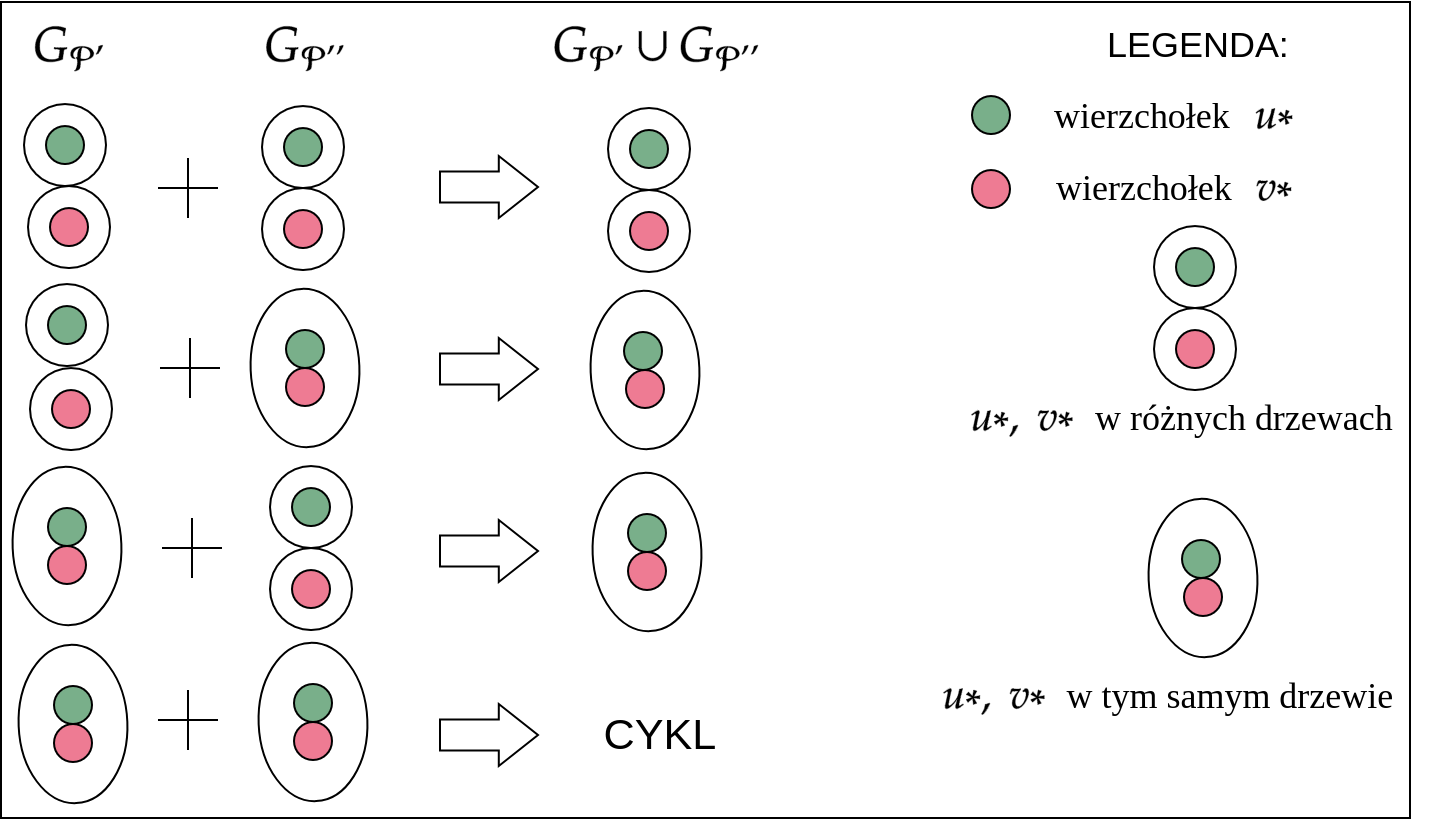
\includegraphics[width=16cm]{find_n_union.png}
\caption{Rezultaty otrzymane w wyniku połączenia lasów $G_{\mathcal{P}'}$, $G_{\mathcal{P}''}$ w węźle scalającym z rys. \ref{dekompozycja_kwadratu}.}
\label{find_n_union}
\end{figure}

$$$$Warunki, które muszą zostać spełnione przy scalaniu dwóch rozwiązań są następujące:
\begin{enumerate}[label=(\roman*)]
\item $G_{\mathcal{P}'} \cup G_{\mathcal{P}''}$ nie zawiera cyklu.
\item $G_{\mathcal{P}'} \cup G_{\mathcal{P}''}$ odpowiada $G_{\mathcal{P}}$ z dokładnością do kształtu poszczególnych drzew. 
\end{enumerate}

W implementacji powyższego algorytmu do reprezentowania problemu łączenia lasów $G_{\mathcal{P}'}$, $G_{\mathcal{P}''}$ wykorzystałam strukturę zbiorów rozłącznych z łączeniem według rangi i kompresją ścieżek. Dzięki niej łatwo wykryć cykl oraz zbadać, które wierzchołki są w tych samych, spójnych komponentach $\mathcal{P}$. Rysunek \ref{find_n_union} przedstawia wszystkie możliwe lasy $G_{\mathcal{P}'}$, $G_{\mathcal{P}''}$ dla węzła scalającego z rysunku \ref{dekompozycja_kwadratu} wraz z rezultatami połączenia lasów.
Końcowe rozwiązanie wyliczamy na podstawie poniższego wzoru:
$$c[t][X][\mathcal{P}] = \min \limits_{\mathcal{P}', \mathcal{P}''} c[t'][X][\mathcal{P}'] + c[t''][X][\mathcal{P}'']$$

Przedstawione zostały formuły rekurencyjne dla wszystkich typów węzłów. Przejdźmy zatem do wyliczenia złożoności czasowej standardowego algorytmu dynamicznego po dekompozycji drzewowej dla problemu drzewa Steinera. Poniżej znajdują się istotne spostrzeżenia:
\begin{enumerate}[label=(\alph*)]
\item Każdy węzeł ma co najwyżek $k+2$ wierzchołki.
\item Wszystkich $X \subseteq X_t$ jest $2^{\abs{X_t}}$ a zatem nie więcej niż $2^{k+2}$.
\item Wszystkich partycji $X$ jest $\abs{X}^{\abs{X}}$ a zatem nie więcej niż $(k+2)^{k+2}$
\item Dla każdego węzła mamy $2^{k+2} \cdot (k+2)^{k+2} = k^{\Omicron(k)}$.
\item Wartości dla każdego węzła wyliczamy w czasie $(k^{\Omicron(k)})^2$.
\end{enumerate}
 
\begin{theorem}
Mając dany $n$-wierzchołkowy graf $G$ razem ze zbiorem terminali $K \subseteq V(G)$ oraz dekompozycją drzewową o szerokości drzewowej nie większej niż $k$, można wyliczyć rozmiar minimalnego drzewa Steinera w czasie $k^{\Omicron(k)} \cdot n$. 
\end{theorem}

    	\section{Cykl Hamiltona}
    	
W tym rozdziale przedstawię klasyczny algorytm dynamiczny po dekompozycji drzewowej dla problemu istnienia cyklu Hamiltona. 

Zakładamy, że mamy daną ładną dekompozycję drzewową lekko zmodyfikowanego grafu $G'$ : $\mathcal{T} = (T, \{X_t\}_{t \in V(T)})$. Modyfikacja polega na tym, że kopiujemy wierzchołek $v_r$, będący w korzeniu dekompozycji drzewowej grafu $G$ (\texttt{ZAPOMINAJĄCY} $v_r$) wraz z jego krawędziami, tj. dla z każdej krawędzi $uv_r \in E(G)$, dostajemy dwie krawędzie $uv_{r_1}$ i $uv_{r_2}$, gdzie $v_{r_1}$ jest byłym wierzchołkiem $v_r$, a $v_{r_2}$ jego kopią. $\mathcal(T)$ nie zawiera węzłów zapominających $v_{r_1}$ oraz $v_{r_2}$. Problem szukania cyklu Hamiltona modyfikujemy do problemu szukania ścieżki Hamiltona o końcach $v_{r_1}$ i $v_{r_2}$.

Ślad cyklu Hamiltona w poddrzewie węzła $t$ składa się ze zbioru rozłącznych ścieżek $F = H \cap G_t = \{C_1, C_2, \ldots, C_z\}$, gdzie $H$ jest szukanym cyklem. $F$ poza liśćmi nie jest puste, ponieważ wszystkie wprowadzone wierzchołki muszą należeć do śladu. Szukane $H$ jest spójne, co implikuje, że każda ścieżka $C_1, \ldots, C_z$ z $F$ przecina $X_t$. Ponadto musi ona przecinać $X_t$ oboma swoimi końcami, wpp. nie dostalibyśmy spójnego rozwiązania końcowego. Z powyższych warunków wynika, że wierzchołki $X_t$ możemy sklasyfikować następująco (rys. \ref{hamiltonian}):
\begin{itemize}[noitemsep,topsep=5pt,parsep=0pt,partopsep=0pt]
\item[$X_{t_0}$] zbiór wierzchołków izolowanych w $F$ (o stopniu $0$)
\item[$X_{t_1}$] zbiór wierzchołków będących końcami ścieżek $C_1, C_2, \ldots, C_z$ (o stopniu $1$)
\item[$X_{t_2}$] zbiór wierzchołków należących do ścieżek $C_1, C_2, \ldots, C_z$ i nie będących ich końcami (o stopniu $2$)
\end{itemize}

\begin{figure}
\centering
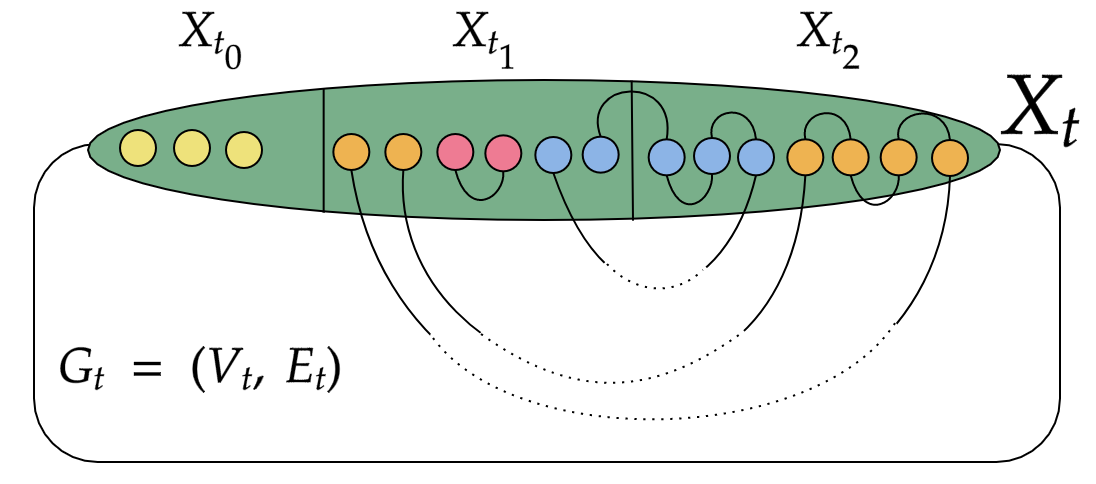
\includegraphics[width=16cm]{hamiltonian.png}
\caption{Przykładowy ślad ścieżki Hamiltona dla węzła $t$.}
\label{hamiltonian}
\end{figure}

Ślad cyklu w węźle $t$ jest jednoznacznie zdefiniowany podziałem zbioru $X_t$ na trzy podzbiory $\mathcal{D} = (X_{t_0}$, $X_{t_1}$, $X_{t_2})$ oraz dopasowaniem $M$. Ślad jest poprawny, jeśli spełnione są poniższe warunki:
\begin{enumerate}[label=(\roman*)]
\item $V(F) = V_t$
\item $u \in X_{t_i}$ $\Leftrightarrow$ $u \in X_t$ i wierzchołek $v$ ma stopień $i$ w $F$
\item $u$ jest skojarzone z $v$ (${u, v} \in M$) $\Leftrightarrow$ $u \in X_{t_1} \wedge v \in X_{t_1} \wedge \exists y: u \in C_y \wedge v \in C_y$ ($u$ i $v$ są końcami ścieżki $C_y$) 
\end{enumerate}  

Dla każdej trójki $(t, \mathcal{D}, M)$ algorytm liczy, czy wyznacza ona poprawny ślad - \emph{true}/\emph{false}. Musimy na bieżąco śledzić dopasowanie $M$, ponieważ węzły typu \texttt{SCALAJĄCY} oraz \texttt{UZUPEŁNIAJĄCY} $uv$ mogą utworzyć cykl. Wynik końcowy odpowiada wartości $c(r, (\emptyset, \{v_1, v_2\}, \emptyset), \{v_{r_1}, v_{r_2}\})$, gdzie $r$ jest korzeniem. Poniżej prezentuję formuły rekurencyjne obliczania wartości $c$ ze względu na typ węzła $t$.
\newline\newline
$t$ jest \texttt{LIŚCIEM}
$$c(t, (\emptyset, \emptyset, \emptyset), \emptyset) = true$$
\newline
$t$ jest węzłem \texttt{WPROWADZAJĄCYM} $v$ - zauważmy, że w momencie dodawania wierzchołka jego stopień wynosi $0$, ponieważ żadna z incydentnych do niego krawędzi nie została jeszcze wprowadzona:

\[
c(t, (X_{t_0}, X_{t_1}, X_{t_2}), M) =  
\left \{
  \begin{tabular}{ccc}
  $c(t', (X_{t_0} \setminus \{v\}, X_{t_1}, X_{t_2}), M)$ & jeśli $v \in X_{t_0}$,\\
  $0$ & wpp.
  \end{tabular}
\right. 
\]
\newline
$t$ jest węzłem \texttt{ZAPOMINAJĄCYM} $v$ - wszystkie krawędzie incydentne do zapominanego wierzchołka zostały już wprowadzone, wobec czego zapominany wierzchołek jest stopnia $2$:

$$c(t, (X_{t\_0}, X_{t\_1}, X_{t\_2}), M) = c(t', (X_{t\_0}, X_{t\_1}, X_{t\_2} \cup \{v\}), M)$$
\newline
$t$ jest węzłem \texttt{WPROWADZAJĄCYM} $uv$ - dodawanie krawędzi incydentnej do wierzchołka zwiększa jego stopień o $1$, wobec czego możemy dodawać krawędź, jeśli $u \in X_{t_0} \vee u \in X_{t\_1}$ oraz $v \in X_{t_0} \vee v \in X_{t_1}$. Nie jest to jednak warunek wystarczający, ponieważ nie gwarantuje nam, że nie dostaniemy cyklu. Jeśli $u \in X_{t_1} \wedge v \in X_{t_1}$ oraz $\exists m : m \in M \wedge u \in m \wedge v \in m$, nie możemy wziąć krawędzi $uv$. Niezależnie od tego, czy krawędź może zostać dodana do rozwiązania, czy nie, dla każdej trójki $(t, \mathcal{D}, M)$ możemy jej nie brać, dlatego bierzemy alternatywę $c(t', (X_{t_0}, X_{t_1}, X_{t_2}), M)$ i poniższych wartości:

\[
c(t, (X_{t_0}, X_{t_1}, X_{t_2}), M) =  
\left \{
  \begin{tabular}{ccc}
  $c(t', (X_{t_0} \cup \{u, v\}, X_{t_1} \setminus \{u, v\}, X_{t_2}), M \cup \{u, v\})$\\
  jeśli $u \in X_{t_1} \wedge v \in X_{t_1}$\\  
  \\
  $c(t', (X_{t_0} \cup \{u\}, X_{t_1} \setminus \{u\} \cup \{v\}, X_{t_2} \setminus \{v\}), M \cup \{u, v\})$\\
  jeśli $u \in X_{t_1} \wedge v \in X_{t_2}$\\
  \\
  $c(t', (X_{t_0} \cup \{v\}, X_{t_1} \setminus \{v\} \cup \{u\}, X_{t_2} \setminus \{u\}), M \cup \{u, v\})$\\
  jeśli $u \in X_{t_2} \wedge v \in X_{t_1}$\\
  \\
  $c(t', (X_{t_0}, X_{t_1} \cup \{u, v\}, X_{t_2} \setminus \{u, v\}), M \cup \{u, v\})$\\
  jeśli $u \in X_{t_2} \wedge v \in X_{t_2}$\\
  \\  
  $0$ wpp.\\
  \end{tabular}
\right. 
\]

\begin{figure}
\centering
\label{hamiltonian_merge}
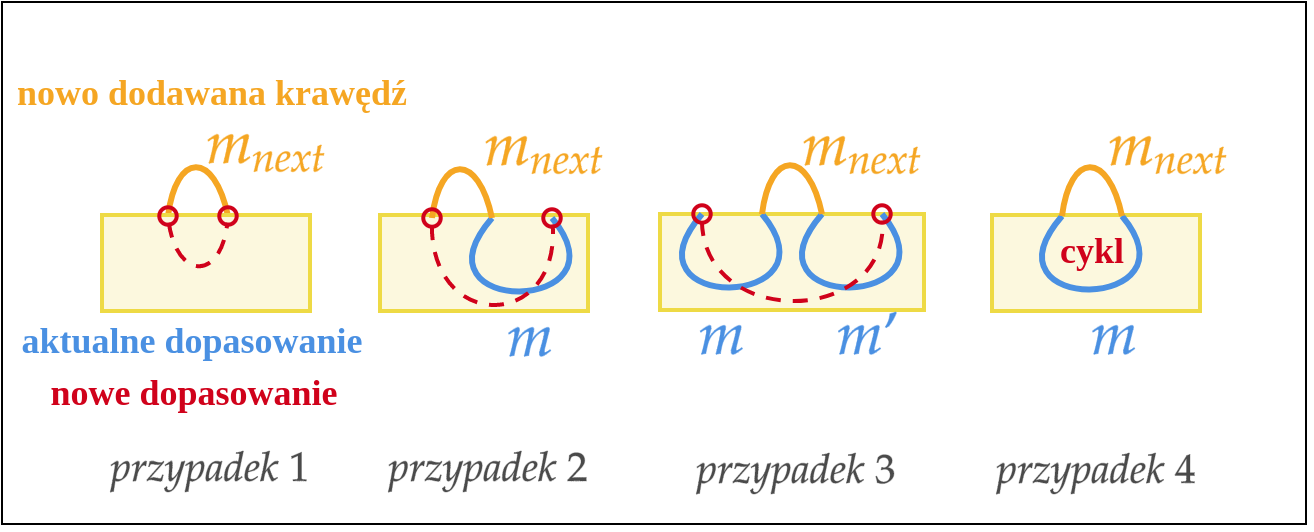
\includegraphics[width=16cm]{hamiltonian_merge.png}
\caption{Dodawanie nowej krawędzi $m_{next}$ do dopasowania $M$.}
\end{figure}
$$$$
$t$ jest węzłem \texttt{SCALAJĄCYM} - zauważmy, że scalane $F_{t'}$ oraz $F_{t''}$ nie mają wspólnych krawędzi, jedynie wierzchołki. Z powyższego wynika, że dla każdego wierzchołka $v$ należącego do $X_t$: $deg_t(v) = deg_{t'}(v) + deg_{t''}(v)$. Zauważmy, że musi być spełniony warunek $deg_t(v) \leq 2$. Jeśli $\mathcal{D}_{t'}$ i $\mathcal{D}_{t''}$ nie spełniają tego warunku, nie rozpatrujemy ich. Jednakże nie jest to warunek wystarczający, by wartość dla węzła $t$ była poprawna. Może się zdarzyć (jak przy dodawaniu krawędzi), że scalanie utworzy nam cykl. Obliczając nowe dopasowanie, dodajemy dopasowania $m_{next} = \{m_{next_1}, m_{next_2}\}$ z $M_{t'} \cup M_{t''}$ pojedynczo, aktualizując obecny stan $M$ w następujący sposób (patrz rys. \ref{hamiltonian_merge}):
\begin{enumerate}
\item $\forall_{m \in M}: m_{next} \cap m = \emptyset$, do dopasowania $M$ dodajemy $m_{next}$.
\item $\exists_{m = \{m_1, m_2\} \in M}: \abs{m_{next} \cap m} = 1 \wedge \forall_{m' \in M, m' \ne m}: m_{next} \cap m' = \emptyset$ - bez straty ogólności załóżmy, że $m_1 = m_{next_1}$, czyli $m_{next} \cap m = \{m_1\}$, z $M$ usuwamy $m$ i dodajemy nowe dopasowanie $\{m_2, m_{next_2}\}$.
\item $\exists_{m = \{m_1, m_2\} \in M}: \abs{m_{next} \cap m} = 1 \wedge \exists_{m' = \{m'_1, m'_2\} \in M, m \ne m'}: \abs{m_{next} \cap m'} = 1$ - bez straty ogólności załóżmy, że $m_{next_1} = m_1$ i $m_{next_2} = m'_1$, usuwamy $m_1$ i $m'_1$ z $M$ oraz dodajemy nowe dopasowanie $\{m_2, m'_2\}$.
\item $\exists_{m \in M}: \abs{m_{next} \cap m} = 2$ - \texttt{CYKL}, $M_{t'}$ i $M_{t''}$ nie utworzą nam poprawnego rozwiązania.
\end{enumerate}

Końcowy wynik dla parametrów $(t, \mathcal{D}, M)$ jest alternatywą po wszystkich $(t', \mathcal{D}_{t'}, M_{t'})$ i $(t'', \mathcal{D}_{t''}, M_{t''})$, które spełniają wyżej wymienione warunki:

$$c[t][\mathcal{D}][M] = \bigvee \limits_{\mathcal{D}_{t'}, \mathcal{D}_{t''}, M_{t'}, M_{t''}} c[t'][\mathcal{D}_{t'}][M_{t'}] \wedge c[t''][\mathcal{D}_{t''}][M_{t''}]$$

Dla każdego węzła mamy nie więcej niż $3^k \cdot k^k$ stanów. Zatem złożoność czasowa standardowego algorytmu dynamicznego po dekompozycji drzewowej dla problemu istnienia cyklu Hamiltona wynosi $k^{\Omicron(k)} \cdot n$, gdzie $n$ jest liczbą wierzchołków grafu $G$ danego na wejściu. 

\newpage
  	\chapter{Algorytmy dynamiczne z zastosowaniem techniki Cut \& Count}

W poprzednim rozdziale zostały przedstawione klasyczne algorytmy dynamiczne po dekompozycji drzewowej dla dwóch problemów decyzyjnych: drzewa Steinera oraz cyklu Hamiltona. Złożoność czasowa obu tych algorytmów jest uwarunkowana liczbą wszystkich możliwych podziałów zbioru $k$-elementowego oraz liczbą dopasowań wierzchołków ze zbioru $k$-elementowego, która w obu przypadkach jest rzędu $k^{\Omicron{(k)}}$.
W tym rodziale przedstawię randomizowane algorytmy dynamiczne po dekompozycji drzewowej, bazujące na technice Cut \& Count opisanej w \emph{Parameterized Algorithms} \cite{parametrized_algorithms}. Technika Cut \& Count redukuje problemy decyzyjne do problemów zliczania wszystkich możliwych rozwiązań modulo $2$, eliminując czynnik $k^{\Omicron{(k)}}$, tym samym znacznie poprawiając złożoność czasową w stosunku do klasycznych algorytmów dynamicznych. Cut \& Count tymczasowo dopuszcza rozwiązania niespójne (las w przypadku drzewa Steinera, zbiór cykli w przypadku cyklu Hamiltona), które następnie wzajemnie się znoszą przy zliczaniu modulo $2$.\newline\newline
Ogólny schemat problemu, który rozwiązujemy z użyciem Cut \& Count przedstawia się następująco: 
Dla uniwersum $U$ niech $\mathcal{S} \subset 2^U$ oznacza zbiór szukanych rozwiązań. Pytamy, czy $\mathcal{S}$ jest pusty.\newline\newline
Technika Cut \& Count bazuje na dwóch operacjach:

\begin{enumerate}

\item[Cut] - poluzuj wymagania dotyczące spójności szukanego rozwiązania, tj. na tym etapie dopuszczamy rozwiązania niespójne należące do zbioru $\mathcal{R} \supseteq \mathcal{S}$. Ponadto rozważamy zbiór $\mathcal{C}$ składający się z par $(X, C)$, gdzie $X \in \mathcal{R}$ a $C$ jest partycją podzbioru wierzchołków grafu wejściowego $(V^1, V^2)$, z którą $X$ jest kompatybilny (żadna spójna składowa nie ma niepustego przecięcia zarówno z $V_1$, jak i $V_2$).  

\item[Count] - wyizoluj jedno z możliwych rozwiązań (o ile takie istnieje) poprzez przypisanie losowych wag elementom z uniwersum $U$. Rozbij zbiór $\mathcal{C}$ ze względu na wagi $w = \mathbf{w}(X)$, a następnie oblicz parzystości zbiorów $\abs{\mathcal{C}_w}$ używając formuł rekurencyjnych. To pozwoli odrzucić wszystkie niepoprawne rozwiązania (niespójne), tj. $X \in \mathcal{R} \setminus \mathcal{S}$, ponieważ każde niespójne rozwiązanie jest kompatybilne z parzystą ilością partycji. Istnienie spójnego, wyizolowanego rozwiązania sprawi, że jedna z wartości $\abs{\mathcal{C}_w}$ będzie równa $1$.

\end{enumerate}

    	\section{Drzewo Steinera}


\begin{theorem}
\label{monte_carlo}
\em Istnieje algorytm Monte Carlo z jednostronnym błędem - algorytm może zwrócić odpowiedź negatywną, kiedy rozwiązanie istnieje - który rozwiązuje problem drzewa Steinera w czasie $3^k \cdot n^{\Omicron(1)}$ mając na wejściu daną dekompozycję drzewową grafu o szerokości drzewowej $k$.
\end{theorem}

\begin{proof}
Jak już zostało wspomniane, sprowadzamy problem decyzyjny do problemu parzystości liczby rozwiązań. Jednakże nie liczymy jej bezpośrednio, a uwzględniając rozwiązania niespójne - jak zostanie to pokazane, każde z nich wliczamy do końcowego wyniku parzystą liczbę razy, dzięki czemu wynik końcowy jest od nich niezależny.

Powołując się na \emph{Parametrized Algorithms} \cite{parametrized_algorithms}, zdefiniujmy dwa zbiory $\mathcal{R}$ i $\mathcal{S}$. $\mathcal{R}$ niech będzie zbiorem ,,lasów Steinera'', tj. zbiorem acyklicznych podgrafów $G$, których suma ma co najwyżej $\ell$ krawędzi i zawiera wszystie terminale $K$. $\mathcal{S}$ niech zawiera te podgrafy z $\mathcal{R}$, które są dodatkowo spójne:

$$\mathcal{R} = \{H \subseteq G: \abs{E(H)} \leq \ell, K \subseteq V(H)\}$$
$$\mathcal{S} = \{H \in \mathcal{R}: H\ jest\ sp\mbox{ó}jny\}$$

Dążymy do tego, by każdy element z $\mathcal{R} \setminus \mathcal{S}$ został zliczony parzystą liczbę razy, natomiast każdy element ze zbioru $\mathcal{S}$ nieparzystą liczbę razy. W tym celu definiujemy rodzinę podziałów zbioru $V(H)$ na dwa podzbiory $V^1$ i $V^2$:
$$\texttt{cuts} (V(H)) \coloneqq \{(V^1, V^2): V^1 \cup V^2 = V(H) \wedge V^1 \cap V^2 = \emptyset\}$$
\begin{definition}
\em \emph{Graf $H$ jest kompatybilny z podziałem $(V^1, V^2)$}, jeśli $E(H) \subseteq {V^1 \choose 2} \cup {V^2 \choose 2}$, gdzie ${X \choose 2}$ oznacza wszystkie dwuelementowe podzbiory zbioru $X$.  
\end{definition}

Zastanówmy się, jak wiele podziałów jest komptybilnych z grafem $H \in \mathcal{R}$. Skoro żadna z krawędzi nie może być rozpięta pomiędzy $V^1$ i $V^2$, każdy spójny komponent $H$ musi być w całości w $V^1$ lub w $V^2$. Z powyższego dostajemy, że dla danego $H$ mamy $2^c$ kompatybilnych podziałów, gdzie $c$ jest liczbą spójnych składowych $H$. Każde niespójne $H$ (z więcej niż jedną spójną składową) jest kompatybilne z parzystą liczbą podziałów, dzięki czemu rozwiązania niespójne się znoszą. Niestety spójne rozwiązania są również kompatybilne z parzystą liczbą podziałów - z dokładnie dwoma. Aby każde spójne rozwiązanie zostało zliczone dokładnie raz, wybieramy dowolny wierzchołek $v_0 \in K$ i przypisujemy go na stałe tylko do $V^1$. Zapiszmy formalnie nową definicję rodziny podziałów $V(H)$:

$$\texttt{cuts} (V(H), v_0) \coloneqq \{(V^1, V^2): V^1 \cup V^2 = V(H) \wedge V^1 \cap V^2 = \emptyset \wedge v_0 \notin V^2\}$$

Pokażę teraz, że zamiast liczyć parzystość $\abs{\mathcal{S}}$, możemy policzyć parzystość zbioru $\mathcal{C}$ zdefiniowanego następująco:
$$\mathcal{C} = \{(H, (V^1, V^2)) \in \mathcal{R} \times \texttt{cuts}(V(H), v_0) : H\ jest\ kompatybilny\ z\ (V^1, V^2)\}$$

\begin{lemma}
Parzystość $\abs{\mathcal{C}}$ jest równa parzytości $\abs{\mathcal{S}}$.
\end{lemma}

\begin{proof}
Rozważmy graf $H$ należący do $\mathcal{R}$, który ma $c$ spójnych składowych. Wiezrchołki każdej spójnej składowej muszą się znaleźć w całości w $V^1$ albo w $V^2$. Jednakże spójna składowa zawierająca $v_0$ może się znaleźć tylko po stronie $V^1$. Z tego powodu $H$ jest kompatybilny z $2^{c-1}$ podziałami. Dla $H \in \mathcal{S}$ liczba ta jest nieparzysta, natomiast dla $H \in \mathcal{R} \setminus \mathcal{S}$ parzysta. 
\end{proof}

Wobec powyższego lematu, pozostaje pokazać algorytm obliczania parzystości $\mathcal{C}$. Dla każdego węzła $t \in V(T)$, liczby naturalnej $i \leq l$ i funkcji $f: X_t \to \{0,1,2\}$ obliczamy $c(t, f, i)$, które równa się liczbie par $(H, (V^1, V^2))$, takich że:

\begin{enumerate}[label=(\roman*)]
\item $H$ jest podgrafem $(V_t, E_t)$ o dokładnie $i$ krawędziach oraz $H$ zawiera wszystkie terminale wprowadzone w bieżącym poddrzewie, tj. $K \cap V_t$.
\item $(V^1, V^2)$ jest przecięciem kompatybilnym z $H$, tj. $(H, (V^1, V^2)) \in \mathcal{C}$.
\item Przecięcie $H$ z wierzchołkami należącymi do węzła $t$ jest równe $V(H) \cap X_t = f^{-1}(1) \cup f^{-1}(2)$.
\item Funkcja $f$ opisuje przynależność wierzchołków ze zbioru $X_t \setminus f^{-1}(0)$ do $V^1$ i $V^2$, tj. $V^j \cap V(H) \cap X_t = f^{-1}(j)$ gdzie $j \in \{1,2\}$.
\end{enumerate} 

Zanim zdefiniuję rekurencyjne formuły obliczania wartości $c(t, f, i)$, pokażę w jaki sposób problem parzystości $\mathcal{C}$ redukuje się do problemu istnienia drzewa Steinera. Oczywistym jest, że może istnieć parzyście wiele różnych drzew Steinera o tej samej liczbie krawędzi, które się wzajemnie zniosą. Problem ten rozwiążemy poprzez wprowadzenie wag na krawędziach grafu $G$, które pozwolą nam rozróżniać poszczególne rozwiązania. 
Dla odpowiednio dużego $N$, losowo (niezależnie i z równym prawdopodobieństwem) wybieramy wagi ze zbioru $\{1,2,\dots,N\}$ i przyporządkowywujemy je krawędziom należącym do $E(G): \mathbf{w}(e) \in \{1,2,\dots,N\}$. 

\begin{definition}
\em \emph{Waga grafu $H$} jest sumą wag wszystkich jego krawędzi:
$$\mathbf{w}(H) = \sum_{e \in E(H)} \mathbf{w}(e)$$
\end{definition}
Dla liczby naturalnej $w$, niech $\mathcal{R}_w = \{H \in \mathcal{R} : \mathbf{w}(H) = w\}$. Podobnie definiujemy $\mathcal{S}_w$ i $\mathcal{C}_w$. Z oczywistych względów $\abs{\mathcal{S}_w} \mod 2 = \abs{\mathcal{C}_w} \mod 2$ oraz zachodzi poniższa implikacja:
\begin{center}
$\exists_{w} :\abs{\mathcal{S}_w} \mod 2 = 1 \implies$ istnieje drzewo Steinera o $i \leq l$ krawędziach.
\end{center}

Intuicyjnie, wystarczająco duże $N$ powinno porozrzucać poprawne rozwiązania do różnych $\mathcal{S}_w$. Z tego wynika, że jeśli istnieje drzewo Steinera o $i \leq l$ krawędziach, to z wysokim prawdopodobieństwem $\exists_{w} :\abs{\mathcal{S}_w} \mod 2 = 1$.
Autorzy udowadniają za pomocą tzw. lematu izolującego coś znacznie silniejszego - mianowicie wystarczy wziąć $N = \Omega(\abs{E(G)})$, żeby ze stałym prawdopodobieństwem otrzymać co najmniej jeden zbiór $\mathcal{S}_w$ rozmiaru dokładnie $1$.

Naszym uniwersum są krawędzie grafu wejściowego $U = E(G)$. Wagi na krawędziach losujemy ze zbioru $\{1,2, \ldots, 2 \abs{U}\}$, a następnie liczymy parzystości $\abs{\mathcal{C}_w}$. Modyfikujemy algorytm, dodając paramter $w$. Algorytm oblicza wartość $c(t, f, i, w)$ równą liczbie podgrafów $H$ o wadze $w$, $i$ krawędziach, kompatybilnych z podziałem $(V_1, V_2)$. Poniżej przedstawiam rekurencyjne formuły zależne od typu węzła $t$. Rozwiązanie końcowe zależy od tego, czy istnieje $i \leq l$ oraz $w  \leq 2\abs{E}l$, dla których  $c[r][0][i][w] \mod 2 = 1$. Jeśli tak, to istnieje drzewo Steinera o $i$ krawędziach. Jeśli nie, to z prawdopodobieństwem co najmniej $\frac{1}{2}$ nie istnieje drzewo Steinera o co najwyżej $l$ krawędziach. 
\newline\newline
$t$ jest \texttt{LIŚCIEM}
$$c[t][\emptyset][0][0] = 1$$
\newline
$t$ jest węzłem \texttt{WPROWADZAJĄCYM} $v$ - zauważmy, że $v \in K \implies f(v) \neq 0$ oraz $v = v_0 \implies f(v) = 1$. Jeśli któryś z wymienionych warunków nie jest spełniony $c[t][f][i][w] = 0$, wpp.

$$c(t,f,i,w) = c(t',f_{\big|X_{t'}},i,w)$$
\newline
$t$ jest węzłem \texttt{ZAPOMINAJĄCYM} $v$ - dla węzła zapominającego sumujemy wyniki z węzła $t'$ po różnych wartościach funkcji $f(v)$: $0$, $1$, $2$.
\[
c(t,f,i,w) =  
  \begin{tabular}{ccc}
  $\ \ c(t',f \cup \{v, 0\},i,w)$\\
  $+ c(t',f \cup \{v, 1\},i,w)$\\
  $+ c(t',f \cup \{v, 2\},i,w)$
  \end{tabular}
\]
\newline
$t$ jest węzłem \texttt{WPROWADZAJĄCYM KRAWĘDŹ} $uv$ - zauważmy, że krawędź $uv$ może zostać dodana do rozwiązania, kiedy parametry $(t,f,i,w)$ opisują stan, w którym $f(u) = f(v) \neq 0$ - $uv$ jest zgodna z podziałem $(V^1, V^2)$ oraz $u$ i $v$ nie są wierzchołkami izolowanymi.
\[
c(t,f,i,w) =  
\left \{
  \begin{tabular}{ccc}
  $c(t',f,i,w) + c(t',f,i-1,w-w_{uv})$, jeśli $f(u) = f(v) \neq 0$ \\
  $c(t',f,i,w)$, wpp. \\
  \end{tabular}
\right. 
\]
$t$ jest węzłem \texttt{SCALAJĄCYM} - dla węzła scalającego wynik jest sumą po wszystkich parach ($\mathcal{C}_{\mathbf{w}(H')}$, $\mathcal{C}_{\mathbf{w}(H'')}$), gdzie $H'$ jest podgrafem $G_{t'}$, a $H''$ podgrafem $G_{t''}$.

$$c(t,f,i,w) = \sum_{i' + i'' = i, \quad w' + w'' = w} c(t',f,i',w') + c(t'',f,i'',w'')$$

Złożoność powyższego algorytmu wynosi $3^k \cdot n^{\Omicron(1)}$, czyli zależność złożoności czasowej od szerokości drzewowej jest rzędu $2^{\Omicron(k)}$, a nie jak w przypadku standardowego algorytmu dynamicznego $k^{\Omicron(k)}$, co kończy dowód twierdzenia \ref{monte_carlo}.
\end{proof}

    	\section{Cykl Hamiltona}

W tym rozdziale przedstawię zastosowanie techniki Cut \& Count do rozwiązania problemu istnienia cyklu Hamiltona. Ponieważ aspekty techniczne w większości pokrywają się z tym, co zostało przedstawione w poprzednim paragrafie dla drzewa Steinera, skupię się wyłącznie na niuansach charakterystycznych dla cyklu Hamiltona.

Pominięcie wymogu spójności redukuje problem cyklu Hamiltona do problemu pokrycia wierzchołkowego grafu $k$ cyklami, gdzie w naszym przypadku $k \in \{1, \ldots, \floor*{\frac{|V|}{2}}\}$. Zbiór $\mathcal{R}$ jest zbiorem pokryć $H$, które składają się z cykli co najmniej dwuelementowych i których suma pokrywa wszystkie wierzchołki grafu $G$:

$$\mathcal{R} = \{H \subseteq G: V(H) = V(G), \forall u \in V(H): deg(u) = 2\}$$
$$\mathcal{S} = \{H \in \mathcal{R}: H\ jest\ sp\mbox{ó}jny\}$$

Zauważmy, że o ile w przypadku problemu drzewa Steinera mamy zachowany niezmiennik, że jego ślad składa się z drzew, o tyle w przypadku cyklu Hamiltona podobny niezmiennik nie zachodzi. Rozwiązanie dla bieżącego podgrafu $G_t$ składa się nie tylko z cykli, ale także ze ścieżek. Zliczamy takie rozwiązania, dopóki istnieje możliwość domknięcia wszystkich ścieżek (tzn. w węźle zapominającym $v$ wymagamy, by $deg(v) = 2$).

Zbiór $\mathcal{C}$ definiujemy podobnie jak dla drzewa Steinera, z dwiema drobnymi modyfikacjami. Jedna z nich dotyczy $v_0$, który dla cyklu Hamiltona jest dowolnym, ale ustalonym wierzchołkiem ze zbioru $V(G)$. Druga natomiast dotyczy podziału $(V^1, V^2)$, który definiujemy tylko na wierzchołkach o stopniu $1$.
$$\texttt{cuts} (V_{deg_1}(H), v_0) \coloneqq \{(V^1, V^2): V^1 \cup V^2 = V_{deg_1}(H) \wedge V^1 \cap V^2 = \emptyset \wedge v_0 \notin V^2\}$$
$$\mathcal{C} = \{(H, (V^1, V^2)) \in \mathcal{R} \times \texttt{cuts}(V_{deg_1}(H), v_0) : H\ jest\ kompatybilny\ z\ (V^1, V^2)\}$$

Zbiory $\mathcal{R}_w$, $\mathcal{S}_w$ oraz $\mathcal{C}_w$ definiujemy analogicznie jak dla problemu drzewa Steinera. Rysunek \ref{cnc_hamiltonian} przedstawia ślad cyklu Hamiltona w węźle $t$. Zbiór $X_t$ jest podzielony na cztery podzbiory składające się z wierzchołków o różnej charakterystyce:
\addtolength{\leftmargini}{3cm}
\begin{itemize}[noitemsep,topsep=5pt,parsep=0pt,partopsep=0pt]
\item[$X_{t_0}$ ] jest zbiorem wierzchołków o stopniu $0$.
\item[$X_{t_{1_1}}$] jest zbiorem wierzchołków o stopniu $1$, należacych do $V^1$.
\item[$X_{t_{1_2}}$] jest zbiorem wierzchołków o stopniu $1$, należących do $V^2$.
\item[$X_{t_2}$ ] jest zbiorem wierzchołków o stopniu $2$.
\end{itemize}
\addtolength{\leftmargini}{-3cm}
\begin{figure}
\centering
\label{cnc_hamiltonian}
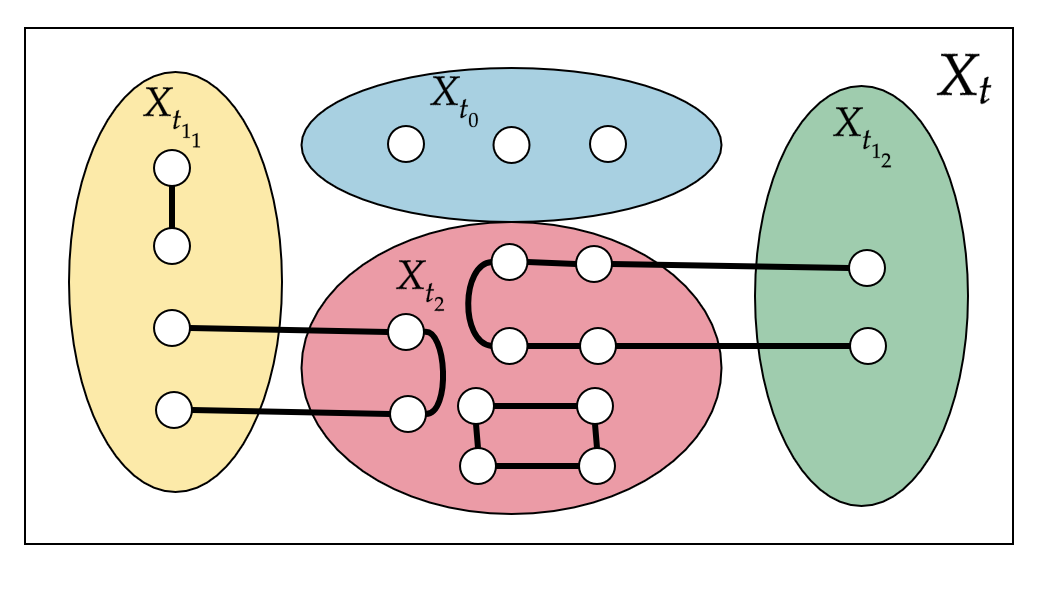
\includegraphics[width=16cm]{cnc_hamiltonian.png}
\caption{$X_t$ ze śladem cyklu Hamiltona.}
\end{figure}
$$$$

Dla każdego węzła $t \in V(T)$, funkcji $f: X_t \to \{0,1_1,1_2,2\}$ oraz wagi $w$ rekurencyjnie obliczamy $c(t,f,w)$ będące liczbą par $(H, (V^1, V^2))$, takich że:

\begin{enumerate}[label=(\roman*)]
\item $H$ jest podgrafem $(V_t, E_t)$ oraz $H$ zawiera wszystkie wierzchołki dotychczasowo wprowadzone w bieżącym poddrzewie, tj. $V(H) = V_t$.
\item $(V^1, V^2)$ jest przecięciem kompatybilnym z $H$.
\item Funkcja $f$ opisuje przynależność wierzchołków ze zbioru $X_t$ do podzbiorów $X_{t_0}, X_{t_{1_1}}, X_{t_{1_2}}, X_{t_2}$, tj. $X_{t_j} \cap V(H) = f^{-1}(j)$, gdzie $j \in \{0,1_1,1_2,2\}$.
\item $X_t = f^{-1}(0) \cup f^{-1}(1_1) \cup f^{-1}(1_2) \cup f^{-1}(2)$
\item $V^1 \cup V^2$ nie ma wierzchołków poza $X_t$, innymi słowy $V_{deg_1}(H) \cap X_t = V_{deg_1}(H)$, inaczej nieodwołalnie zostawilibyśmy niedomknięty cykl.
\item $X_{t_{1_1}} = V^1$ oraz $X_{t_{1_2}} = V^2$
\item $v \in X_{t_j} \implies deg(v) = j$ dla $j \in \{0,1,2\}$
\item $\sum_{e \in E(H)} \mathbf{w}(e) = w$
\end{enumerate}

Zauważmy, że każdy wierzchołek musi po kolei należeć do $X_{t_0} \to \{X_{t_{1_1}} \ lub \ X_{t_{1_2}}\} \to X_{t_2}$. Poniżej przedstawiam definicje rekurencyjne obliczania wartości $c(t,f,w)$. Algorytm zwraca, że istnieje cykl Hamiltona, jeśli $\exists_{w \leq nN}: c(r,\emptyset,w) \mod 2 = 1$, gdzie $r$ jest korzeniem dekompozycji drzewowej, a $n = \abs{V(G)}$.
\newline\newline
$t$ jest \texttt{LIŚCIEM}
$$c(t,\emptyset,0) = 1$$
\newline
$t$ jest węzłem \texttt{WPROWADZAJĄCYM} $v$ - wierzchołek $v$ w momencie wprowadzania nie ma incydentnej krawędzi, zatem jeśli $f(v) \neq 0$, to $c(t,f,w) = 0$, wpp.
$$c(t,f,w) = c(t',f_{\big|X_{t'}},w)$$

\begin{table}
\centering
\begin{tabular}{c|c|c|c|c}
 & $X_{t'_0}$ & $X_{t'_{1_1}}$ & $X_{t'_{1_2}}$ & $X_{t'_2}$ \\
\hline
$X_{t'_0}$ & $(1_1,1_1) \vee (1_2,1_2)$ & $(1_1,2)$ & $\emptyset$ & $(1_2,2)$ \\
\hline
$X_{t'_{1_1}}$ & $(2,1_1)$ & $(2,2)$ & $\emptyset$ & $\emptyset$ \\
\hline
$X_{t'_{1_2}}$ & $\emptyset$ & $\emptyset$ & $\emptyset$ & $\emptyset$ \\
\hline
$X_{t'_2}$ & $(2,1_2)$ & $\emptyset$ & $\emptyset$ & $(2,2)$ \\
\end{tabular}
\caption{Tabela przedstawia, jak zmienia się przynależność wierzchołków $u$ i $v$ do zbiorów $X_{t_i}$ po połączeniu ich krawędzią. Tabelę należy rozumieć w następujący sposób: $tab[f'(u)][f'(v)] = (f(u), f(v))$, $i$ jest tożsame z $X_{t_i}$, a $f'$ odpowiada funkcji $f$ w węźle $t'$.}
\label{add_edge_table}
\end{table}
$$$$
$t$ jest węzłem \texttt{ZAPOMINAJĄCYM} $v$ - wierzchołek może zostać zapomniany wtw. gdy znajduje się w $X_{t_2}$, czyli ma dwie incydentne krawędzie, jeśli $f(v) \neq 2$, to $c(t,f,w) = 0$, wpp.
$$c(t,f,w) = c(t',f \cup \{(v,2)\},w)$$
\newline
$t$ jest węzłem \texttt{WPROWADZAJĄCYM KRAWĘDŹ} $uv$ - następujące warunki muszą być spełnione, żeby można było dodać krawędź $uv$:
\begin{enumerate}[label=(\roman*)]
\item \label{wpr_kr_i}$deg(u) < 2$ oraz $deg(v) < 2$
\item \label{wpr_kr_ii}$uv$ jest kompatybilna z podziałem $(V^1, V^2)$.
\item \label{wpr_kr_iii}$tab[f'(u)][f'(v)] \neq -$, gdzie $tab$ odnosi się do tabeli \ref{add_edge_table}.  
\end{enumerate}

\[
c(t,f,w) =  
\left \{
  \begin{tabular}{ccc}
  $c(t',f,w) + c(t',f',w - w_{uv})$, & jeśli spełnione są warunki \ref{wpr_kr_i}, \ref{wpr_kr_ii}, \ref{wpr_kr_iii}\\
  $c(t',f,w)$, &  wpp.
  \end{tabular}
\right. 
\]

\begin{table}
\centering
\begin{tabular}{c|c|c|c|c}
 & $X_{t''_0}$ & $X_{t''_{1_1}}$ & $X_{t''_{1_2}}$ & $X_{t''_2}$ \\
\hline
$X_{t'_0}$ & $0$ & $1_1$ & $2$ & $1_2$ \\
\hline
$X_{t'_{1_1}}$ & $1_1$ & $2$ & $-$ & $-$ \\
\hline
$X_{t'_{1_2}}$ & $2$ & $-$ & $-$ & $-$ \\
\hline
$X_{t'_2}$ & $1_2$ & $-$ & $-$ & $2$ \\
\end{tabular}
\caption{Zmiana przynależności wierzchołka do zbioru $X_{t_i}$ po scaleniu dwóch podgrafów. Tabelę należy interpretować następująco: $tab[f'(v)][f''(v)] = f(v)$, $i$ jest tożsame z $X_{t_i}$, $f'$ i $f''$ odpowiadają funkcji $f$ w węzłach $t'$ i $t''$.}
\label{merge_table}
\end{table}
$$$$
$t$ jest węzłem \texttt{SCALAJĄCYM} - żeby otrzymać poprawne rozwiązanie w wyniku scalenia, muszą zachodzić następujące warunki:
\begin{enumerate}[label=(\roman*)]
\item \label{scal_i}$\forall v \in X_t$: $deg_{t'}(v) + deg_{t''}(v) \leq 2$
\item \label{scal_ii}$\forall v \in X_t$: jeśli $v \in X_{t'_{1_1}}$, to $v \notin X_{t''_{1_2}}$
\item \label{scal_iii}$tab[f'(v)][f''(v)] \neq -$, gdzie $tab$ odnosi się do tabeli \ref{merge_table}.
\end{enumerate}

\[
c(t,f,w) =  
\left \{
  \begin{tabular}{ccc}
  $\sum_{w' + w'' = w} c(t',f',w') + c(t'',f'',w'')$, & jeśli spełnione są warunki \ref{scal_i}, \ref{scal_ii}, \ref{scal_iii}\\
  0, & wpp. \\
  \end{tabular}
\right. 
\]

Złożoność powyższego algorytmu wynosi $4^k \cdot n^{\Omicron(1)}$, czyli zależność złożoności czasowej od szerokości drzewowej jest rzędu $2^{\Omicron(k)}$, a nie jak w przypadku standardowego algorytmu dynamicznego $k^{\Omicron(k)}$.

\newpage
	\begin{thebibliography}{9}
		\bibitem{bodlaender}  
			H. L. Bodlaender. 
			\textit{A linear-time algorithm for finding tree-decompositions of small treewidth}. 
			SIAM J. Comput. 25:6 (1996) 1305-1317		
		
		\bibitem{kloks} 
			T. Kloks. 
			\textit{Treewidth. Computations and approximations}. 
			Lecture Notes in Computer Science, 842, 1994.
			
		\bibitem{parametrized_algorithms}
			M. Cygan, F. V. Fomin, Ł. Kowalik, D. Lokshtanov, D. Marx, M. Pilipczuk, M. Pilipczuk, S. Saurabh
 			\textit{Parameterized Algorithms}.
 			
		\bibitem{github} 
			P. Kyzioł: Cut \& Count - Code repository, 2019
			\\\texttt{https://github.com/polapl/Cut-and-Count}
	\end{thebibliography} 



\end{document}
